\subsection{Root Finding Problem}
    Every nonlinear equation $g(x) = h(x)$ can be written as $g(x) - h(x) = f(x) = 0$ $\Rightarrow$ We transform the problem into a root finding problem for $f(x)$: find $x^\star$ s.t.
    \begin{equation*}
        \colorboxed{red}{
        \begin{aligned}
            f(x^\star) &= 0\\
            e_k = x_k -x^\star &\ \big(\approx x_k -x_{k-1}\big)
        \end{aligned}
        }
    \end{equation*}
    There is no general formula to find a root of a nonlinear function $\rightarrow$ iterative methods that, from an initial guess $x_0$, produce a sequence $x_0, x_1, \dots, x_k$ that converges to $x^\star$ for $k\to\infty$.
    
    % \subsubsection{Existence of a root}
    %     \begin{itemize}
    %         \item \textit{Intermediate Value Theorem:} If $f$ continuous on $[a,b]$, $\exists x^\star$ s.t. $f(x^\star)=y$ $ \forall y\in [f(a),f(b)]$
    %         \item \textit{Bolzano's Theorem:} If $f$ continuous on $[a,b]$ and $\textrm{sign}(f(a)) \neq \textrm{sign}(f(b))$, $\exists x^\star$ s.t. $f(x^\star)=0$
    %     \end{itemize}
        
    \subsubsection{Sensitivity and Conditioning}
        \textit{If $|f(\Tilde{x})|\approx 0$ does this mean that $|\Tilde{x}-x^\star|\approx0$?}
        We call a system ($f$) \textbf{well-conditioned} when a small change in input causes a small change in the output. \textbf{Ill-conditioned} if small change in input causes a large change in output.
        
        Condition number of root finding problem:
        \begin{equation*}
            \colorboxed{red}{
                \kappa = \frac{1}{|f'(x^\star)|}
            }
        \end{equation*}
        
        If $f'(x)=0$ the problem is ill-conditioned. This is the case for roots with \textbf{multiplicity m} $> 1$.
        
        \subsubsection{Order of Convergence}
            We want the sequence $\{x_k\}_{K=0}^{\infty}$ to converge to $x^\star$ as quick as possible. In order to quantify "\textit{fast}" we define the order of convergende as
            \begin{equation*}
                \lim_{k\to\infty}\frac{|e_{k+1}|}{|e_k|^r}= C
            \end{equation*}
            \textbf{order of convergence} $r$ and \textbf{rate of convergence} $C$
            \begin{itemize}
                \item $r=1$: if $C\in(0,1)$ linear convergence. If $C = 0$ superlinear, $C = 1$ sublinear
                \item $r=2$: quadratic convergence
            \end{itemize}{}

\subsection{Bisection Method}
    \begin{center}
        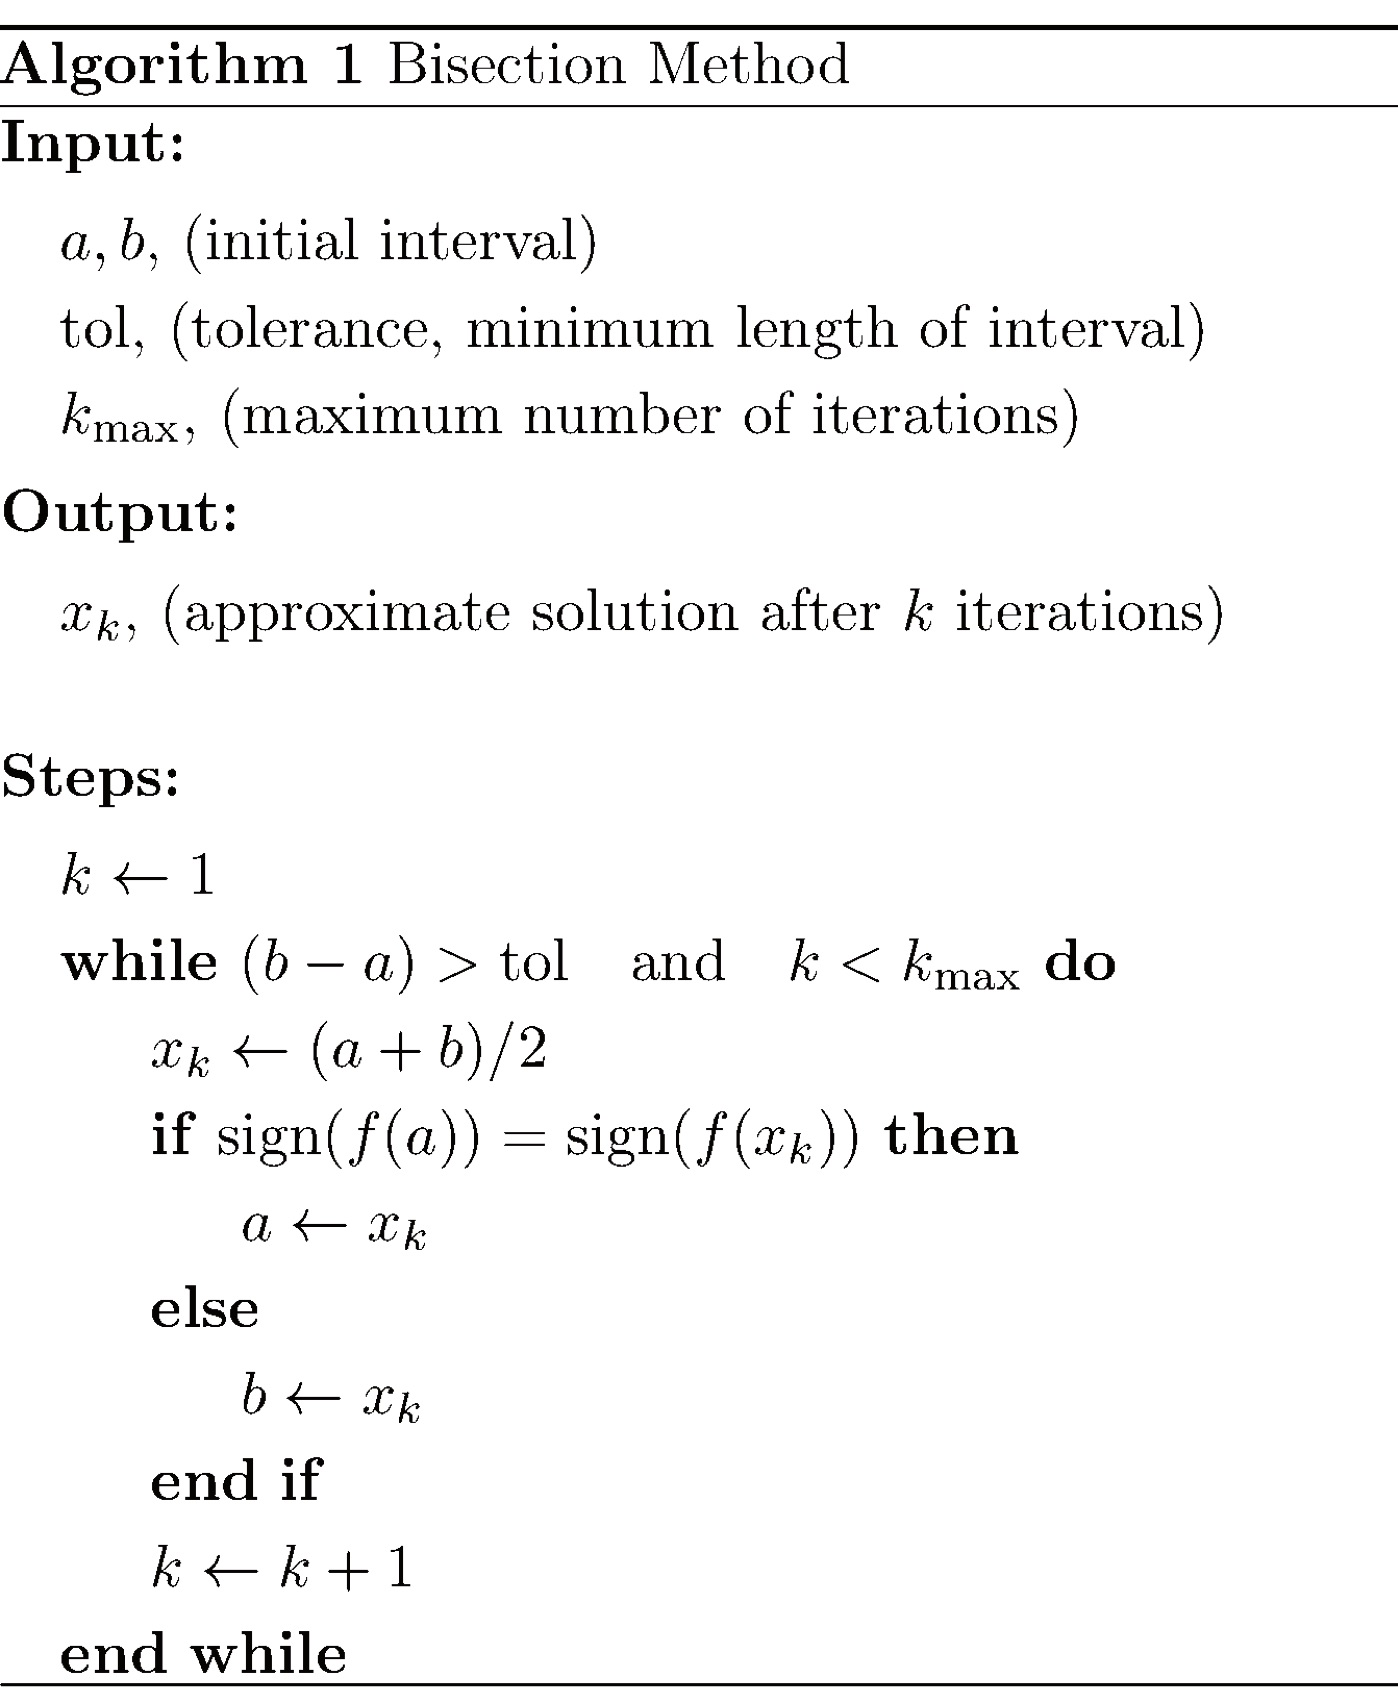
\includegraphics[width=0.9\linewidth, height = 50mm]{images/02/bisection.jpg}
    \end{center}
    Order of convergence: 1 and rate of convergence. $1/2$
    
    Require number of iterations $k$ to achieve tequired tolerance tol.
    \begin{equation*}
        |e_k| = \textrm{tol} \Rightarrow \frac{b-a}{2^k}=\textrm{tol} \Rightarrow k = \log_2\left(\frac{b-a}{\textrm{tol}}\right)
    \end{equation*}
    \textbf{Advantages:}
    \begin{itemize}
        \item Certain to converge
        \item Only requires signs and not function values
        \item $f$ does not need to be differentiable only continuous
    \end{itemize}
    
    \textbf{Disadvantages:}
    \begin{itemize}
        \item Convergence is slow
        \item Initial interval needs to be known beforehand
        \item Cant be easily generalized to higher dimensions
    \end{itemize}



\subsection{Newtons Method}
    Function $f$ continuous and differentiable at $x^\star$.
    \begin{equation*}
        \colorboxed{red}{x_{k+1} = x_k - \frac{f(x_k)}{f'(x_k)}} \ \underbrace{x_{k+1} = x_k - m\frac{f(x_k)}{f'(x_k)}}_{\textnormal{roots with multiplicity }m>1}
    \end{equation*}
    \textbf{Advantages:}
    \begin{itemize}
        \item Quadratic convergence
    \end{itemize}
    
    Newtons method converges quadratically if:
    \begin{equation*}
        \lim_{k\to\infty}\frac{|e_{k+1}|}{|e_k|^2} = \lim_{k\to\infty}\frac{|f''(\xi_k|)}{2|f'(x_k)|}=\frac{|f''(x^\star)|}{2|f'(x^\star)|}=C<\infty
    \end{equation*}
    
    \textbf{Disadvantages:}
    \begin{itemize}
        \item Small changes in IV may change root
        \item\textbf{Root with multiplicity $m>1$ convergence rate only linear}
        \item Not guaranteed to converge
        \item if $f'(x_k)=0$ for some $k$ we cannot proceed
        \item requires evaluation of both $f(x_k)$ and $f'(x_k)$
    \end{itemize}
    \begin{center}
    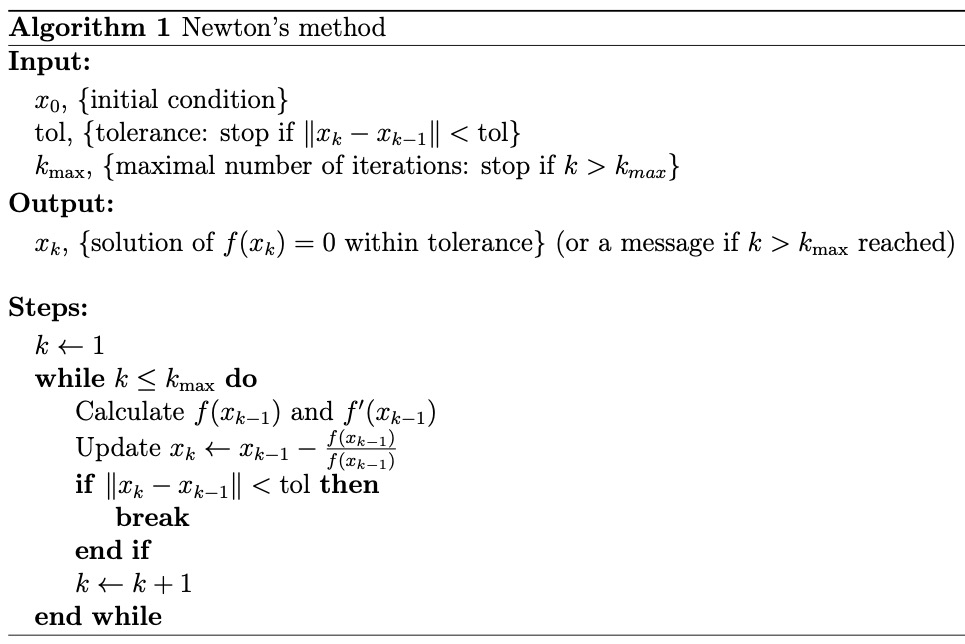
\includegraphics[width=\linewidth]{images/02/newtons_method.jpg} 
    \end{center}
    
\subsection{Secant Method}
    Modification of Newtons method by approximating $f'(x_k) \approx \frac{f(x_k)-f(x_{k-1})}{x_k-x_{k-1}}$
    \begin{equation*}
        \colorboxed{red}{x_{k+1} = x_k - f(x_k)\frac{x_k-x_{k-1}}{f(x_k)-f(x_{k-1})}}
    \end{equation*}
    Order of convergence: $\varphi = \frac{1+\sqrt{5}}{2} \approx 1.618$ (simple roots).
    
    \textbf{Advantages:}
    \begin{itemize}
        \item Avoid evaluation of derivative
        \item Only one function evaluation at each step
    \end{itemize}
    \textbf{Disadvantages:}
    \begin{itemize}
        \item Convergence rate is not quadratic
        \item Needs two initial approximations
    \end{itemize}
    
\subsection{Numerical Computation of the Order of Convergence}
    Compute the error $e_k = x_k-x^\star \, \forall k$ for a function with known root $x^\star$. Then, evaluate the convergence rate $r_k$ as a sequence which will converge to the theoretical $r$.
    \begin{equation*}
        \colorboxed{red}{r \approx \frac{\log\left|\frac{e_{k+2}}{e_{k+1}}\right|}{\log\left|\frac{e_{k+1}}{e_{k}}\right|}} \ \textnormal{log base 10}
    \end{equation*}

